% Phần II: học sinh. Chương 10–14 nối số với Phần I.

\trangphan{hs}{Phần II}{Dành cho học sinh}{Đăng nhập, làm bài, hỏi Kriky những câu em làm sai rồi làm
lại để gỡ điểm.}{\item Đăng nhập \item Làm bài \item Xem kết quả và hỏi Kriky \item Làm lại câu sai
\item Khi gặp trục trặc}

\chapter{Đăng nhập}
\label{chuong:dang-nhap-hs}

Em mở địa chỉ trang học sinh: \diachihocsinh. Tên đăng nhập và mật khẩu do thầy cô phát cho em.

\viec{Đăng nhập}

\anh[0.6\linewidth]{S/01-dang-nhap}{
  \diem{1}{0.035}{0.38}
  \diem{2}{0.035}{0.64}
  \diem{3}{0.035}{0.84}
}

\begin{buoc}
  \item Gõ \nhan{Tên đăng nhập} thầy cô phát, ví dụ \go{khangtm}.
  \item Gõ \nhan{Mật khẩu}.
  \item Bấm \nut{Đăng nhập}.
\end{buoc}

\xong{em thấy trang \nhan{Bài của tôi}, góc phải có tên, lớp và mã của em.}

\luuy{Quên mật khẩu thì nhờ thầy cô đặt lại. Em chưa tự đổi mật khẩu được.}

\machnho{Làm bài trên máy dùng chung thì bấm \nut{Đăng xuất} ở góc phải khi xong.}

\chapter{Làm bài}
\label{chuong:lam-bai}

\viec{Tìm bài cần làm}

\anh{S/02-bai-cua-toi}{
  \diem{1}{0.6}{0.81}
  \diem{2}{0.85}{0.81}
}

Mỗi bài ghi môn, số câu, thời gian làm, hạn vào làm và hạn chữa. Nhãn \sobuoc{1} cho biết em làm được gì;
nút \sobuoc{2} là việc em làm tiếp.

\begin{bangtra}{L{4.6cm}Y}{\dau{Nhãn} & \dau{Nghĩa là}}
  \nhan{Chưa tới giờ mở} & Chưa làm được. Đợi tới giờ thầy cô mở. \\
  \nhan{Đang mở} & Bấm \nut{Bắt đầu} để làm. \\
  \nhan{Đang làm} & Em đã bắt đầu; bấm \nut{Tiếp tục}. \\
  \nhan{Cần làm lại 2 câu} & Em còn câu sai gỡ điểm được (Chương~\ref{chuong:lam-lai}). Nếu chỉ có nút
  \nut{Xem kết quả} thì đã qua hạn làm lại. \\
  \nhan{Đã hoàn thành} & Đã xong hết. Bấm \nut{Xem kết quả}. \\
  \nhan{Hết hạn làm lại} & Đã qua hạn chữa. Vẫn xem được kết quả. \\
  \nhan{Đã đóng} & Đã qua giờ đóng mà em chưa làm. \\
\end{bangtra}

\viec{Bắt đầu làm bài}

\anh[0.5\linewidth]{S/03-bat-dau}{}

Bấm \nut{Bắt đầu}, đọc hộp \nhan{Bắt đầu làm bài?} rồi bấm \nut{Bắt đầu làm bài}. Chưa sẵn sàng thì bấm
\nut{Để sau}.

\luuy{Đồng hồ không dừng được, kể cả khi em đóng trang.}

\viec{Chọn đáp án}

\anh{S/04-lam-bai}{
  \diem{1}{0.015}{0.62}
}

\anh[0.5\linewidth]{S/04b-dong-ho}{
  \diem{2}{0.035}{0.12}
  \diem{3}{0.035}{0.45}
  \diem{4}{0.035}{0.83}
}

\begin{buoc}
  \item Bấm vào phương án em chọn. Đổi ý thì bấm phương án khác.
  \item Theo dõi đồng hồ \nhan{Còn lại}.
  \item Bấm các ô số để sang câu khác. Ô đậm là câu đang xem, ô xanh nhạt là câu đã trả lời, ô xám là câu
        chưa làm. Dòng \nhan{CÒN 3 CÂU CHƯA TRẢ LỜI} đếm số câu còn bỏ trống.
  \item Làm xong thì bấm \nut{Nộp bài}.
\end{buoc}

\viec{Nộp bài}

\anh[0.6\linewidth]{S/05-nop-bai}{}

Hộp \nhan{Nộp bài?} đếm lại số câu đã trả lời. Còn câu chưa làm thì bấm \nut{Quay lại làm tiếp}; xong rồi
thì bấm \nut{Nộp bài}.

\luuy{Nộp rồi thì không sửa được nữa. Câu bỏ trống tính là sai.}

\luuy{Đồng hồ về \nhan{00:00} thì em không chọn thêm được nữa. Bấm \nut{Nộp bài} ngay: bài lần đầu
\textbf{không tự nộp}, và chưa nộp thì chưa có kết quả, chưa chữa được.}

\chapter{Xem kết quả và hỏi Kriky}
\label{chuong:hoi-kriky}

Nộp bài xong, em thấy ngay kết quả. Câu sai chưa phải là hết: em hỏi Kriky cho hiểu, rồi làm một câu
tương tự để gỡ điểm. Hình~\ref{fig:vong-chua-bai} là vòng ấy.

\begin{figure}[htbp]
  \centering
  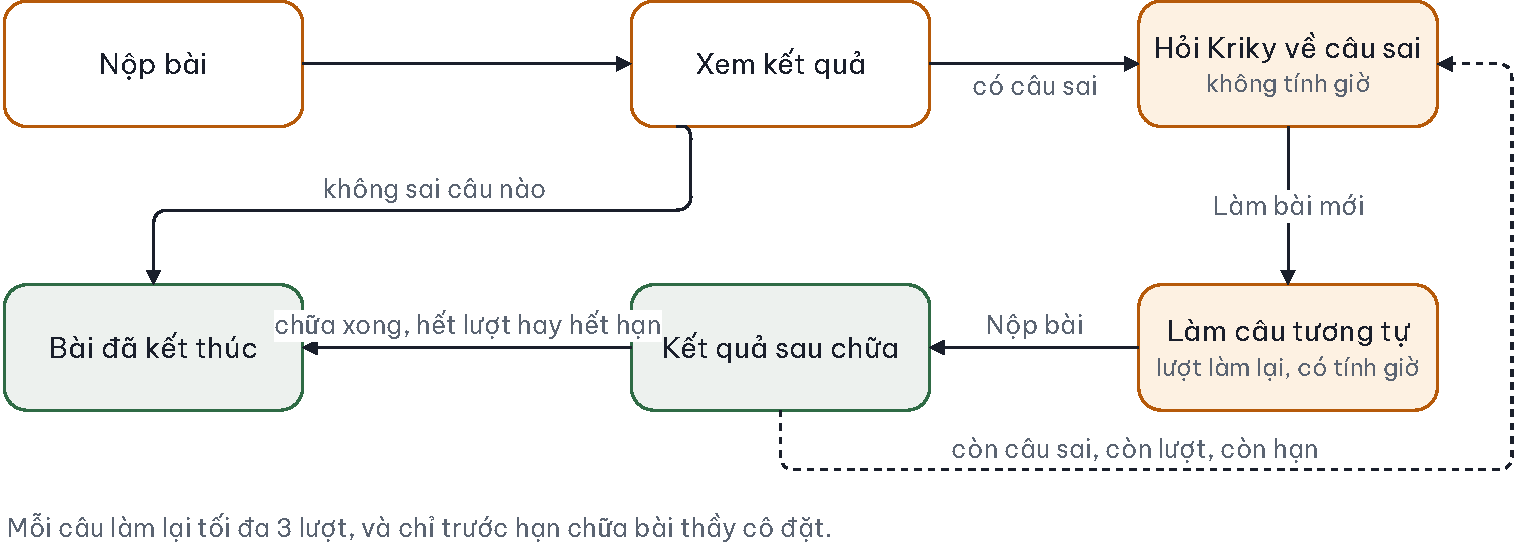
\includegraphics[width=0.9\linewidth]{vong-chua-bai.pdf}
  \caption[Vòng chữa bài]{Vòng chữa bài: hỏi Kriky, làm câu tương tự, tới khi đúng hoặc hết lượt.}
  \label{fig:vong-chua-bai}
\end{figure}

\viec{Xem kết quả}

\anh{S/06-ket-qua}{
  \diem{1}{0.9}{0.86}
  \diem{2}{0.67}{0.09}
}

\begin{buoc}
  \item Câu có vòng tròn rỗng và số 0 bên phải là câu sai; chấm xanh đặc là câu đúng.
  \item Bấm \nut{Hỏi trợ lý và làm lại dạng bài sai} để chữa các câu sai.
\end{buoc}

\machnho{Điểm lúc nộp là điểm sàn. Chữa đúng câu sai trước hạn thì điểm còn tăng.}

\viec{Hỏi Kriky}

\anh[0.6\linewidth]{S/07-hoi-kriky}{}

Gõ câu hỏi vào ô \nhan{Hỏi Kriky về bất kỳ câu nào bạn làm sai…} rồi bấm \nut{Gửi}. Hỏi bằng lời bình
thường, ví dụ:

\begin{loinhan}
Vì sao câu 3 là cực đại mà không phải cực tiểu ạ?
\end{loinhan}

Phần hỏi Kriky không tính giờ. Hỏi tới khi hiểu rồi hãy làm bài mới.

\anh[0.62\linewidth]{S/07b-cau-sai}{
  \diem{1}{0.42}{0.52}
}

Cột bên phải liệt kê \nhan{CÁC CÂU EM LÀM SAI}: em đã chọn gì, đáp án đúng là gì. Bấm \nut{Xem lời giải
đầy đủ ›} \sobuoc{1} để đọc lời giải.

\anh[0.8\linewidth]{S/08-loi-giai}{}

Hộp lời giải có các cách giải và \nhan{ĐỐI CHIẾU TỪNG PHƯƠNG ÁN}: vì sao mỗi phương án đúng hay sai. Bấm
\nut{Đóng} khi xong.

\viec{Báo khi Kriky giải thích khó hiểu}

Khi Kriky đã trả lời câu hỏi đầu tiên của em, nút \nut{Báo cáo Trợ lý giải thích khó hiểu} hiện dưới ô
nhắn. Bấm nút ấy nếu em vẫn chưa hiểu; thầy cô sẽ thấy báo cáo của em.

\anh[0.62\linewidth]{S/09-bao-cao}{}

\xong{nút đổi thành \nhan{Đã báo cho giáo viên}.}

\chapter{Làm lại câu sai}
\label{chuong:lam-lai}

\viec{Bắt đầu lượt làm lại}

\anh[0.6\linewidth]{S/10-bat-dau-lam-lai}{
  \diem{1}{0.972}{0.853}
}

Ở trang hỏi Kriky, bấm \nut{Làm bài mới · 2 câu · 4 phút} (số câu, số phút đổi theo bài). Đọc hộp
\nhan{Bắt đầu lượt làm lại?} (hộp gọi mỗi lượt là một \emph{vòng}) rồi bấm \nut{Làm bài mới} \sobuoc{1}.

Lỡ đóng trang khi đang làm lượt làm lại thì vào lại trang hỏi Kriky: nút đổi thành \nut{Làm tiếp lượt
đang mở}.

\luuy{Bấm là đồng hồ chạy ngay. Gần tới hạn làm lại thì lượt có thể bị dừng giữa chừng.}

\viec{Làm và nộp lượt làm lại}

\anh{S/11-lam-lai}{}

Mỗi câu sai được thay bằng một câu cùng dạng. Em làm như lúc làm bài: chọn đáp án, bấm ô số để sang câu
khác (ô số mang số câu gốc, ví dụ 3 và 6), rồi bấm \nut{Nộp bài}.

\anh[0.6\linewidth]{S/11b-nop-luot}{}

Hộp \nhan{Nộp lượt này?} hỏi lại một lần. Bấm \nut{Nộp bài} để nộp.

\machnho{Hết giờ mà em chưa nộp thì lượt làm lại tự nộp (đã đóng trang thì lượt nộp khi em mở lại).
Câu bỏ trống tính là sai.}

\viec{Xem kết quả sau khi chữa}

\anh{S/12-ket-qua-sau-chua}{}

Câu đã chữa ghi \nhan{Lượt làm lại} và điểm mới. Làm đúng câu tương tự thì câu ấy được 0,5 điểm (nửa
điểm), không phải 1.

\begin{bangtra}{L{5.2cm}Y}{\dau{Em thấy} & \dau{Nghĩa là}}
  Lượt làm lại sai, còn lượt và còn hạn & Hỏi Kriky thêm rồi bấm \nut{Làm bài mới} lần nữa. \\
  Rê chuột lên điểm của câu thấy \nhan{Đã dùng hết ba lượt làm lại cho câu này.} & Câu ấy không chữa
  được nữa. \\
  Bài ghi \nhan{Bài đã kết thúc} & Hết hạn, đã chữa xong hoặc hết lượt. Bấm \nut{Xem lại phần chữa các câu
  sai} để đọc lại. \\
\end{bangtra}

\chapter{Khi gặp trục trặc}

\begin{bangtra}{L{6cm}Y}{\dau{Em thấy} & \dau{Làm gì}}
  Không đăng nhập được & Kiểm tra lại tên đăng nhập, mật khẩu. Vẫn không được thì nhờ thầy cô đặt lại
  mật khẩu. \\
  Không thấy bài thầy cô nói & Hỏi thầy cô bài đã phát hành cho lớp em chưa, hay thầy cô đã thu bài
  về. \\
  \nhan{Bạn nhập sai quá nhiều lần. Thử lại sau N phút.} & Đợi đủ số phút rồi đăng nhập lại. \\
  \nhan{Chưa tới giờ mở} & Đợi tới giờ mở rồi tải lại trang. \\
  Lỡ đóng trang khi đang làm bài & Mở lại trang, bấm \nut{Tiếp tục}. Đồng hồ vẫn chạy trong lúc ấy. \\
  Lỡ đóng trang khi đang làm lượt làm lại & Vào trang hỏi Kriky, bấm \nut{Làm tiếp lượt đang mở}. \\
  Đồng hồ về \nhan{00:00}, bài vẫn \nhan{Đang làm} & Bấm \nut{Nộp bài}. Bài lần đầu không tự nộp. \\
  \nhan{Lượt chữa vừa rồi đã hết giờ nên được nộp luôn…} & Lượt làm lại hết giờ. Câu bỏ trống tính là
  sai; còn lượt thì làm lại. \\
  Nút \nut{Gửi} hỏi Kriky bị khoá & Bài đã kết thúc; em vẫn đọc lại được phần chữa. \\
  Màn hình không cập nhật & Tải lại trang (F5). \\
\end{bangtra}
